\chapter{Online planning}\label{chap:online planning}

\section{ Simulation }
The simulation is done online, but seeks to reduce the output to a minimum. The
main task is to visit all cells in the map and sweep them. This is simulated as
an online statemachine changing between different brahaviours of the robot.

\subsection{Behaviours}
There are basically three beahaviours of the robot:

\begin{itemize}
  \item Select a destination
  \item Go to a destination
  \item Cover a cell
\end{itemize}

The main task is solved using theese three behaviours encapsulated in a state
machine. The state machine concists of two parts. The first part is a decision
maker that selects a route and the other is an onlie stepper to follow the
route.

\subsection{The decision maker}
The decision maker selects a route based on the current state and is thus a
state machine. In either state it facilitates the behaviours to select a route
implemented as a list of points to visit followed by a state transition based on
state variables. The state machine follows the diagram in figure
\ref{fig:decisionmaker}.

\begin{figure}[htb]
	\centering
	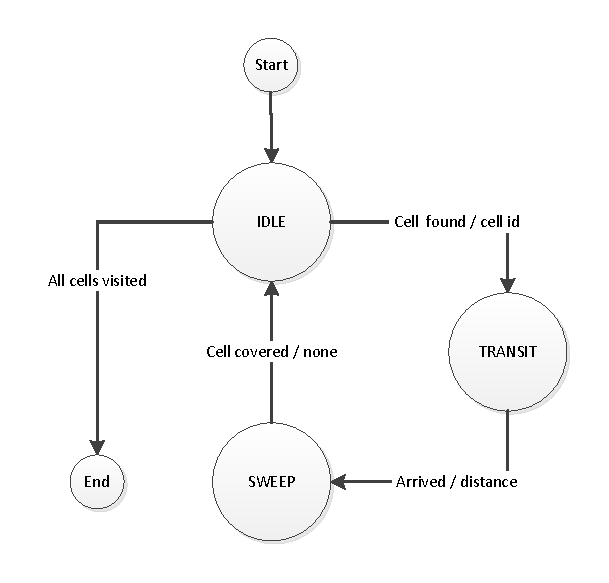
\includegraphics[width=\textwidth,trim=0 0 0 0]{graphics/decisionmaker.pdf}
	%trim=l b r t (can cut off from every side)
	\caption{State machine diagram of the decision maker}
	\label{fig:decisionmaker}			
\end{figure}

\subsection{The stepper}
The stepper is a sequential piece of code that iterates through the list of
points adding up the travelled distance, checking for cups in range, collects
the cups and returns the cups when tray is full. The task of returning the cups
only contributes to the travelled distance since the robot cannot collect cups
and the concept is therefore implemented as a mere calculation. A flow chart for the stepper can be seen in
figure
\ref{fig:stepper}

\begin{figure}[htb]
	\centering
	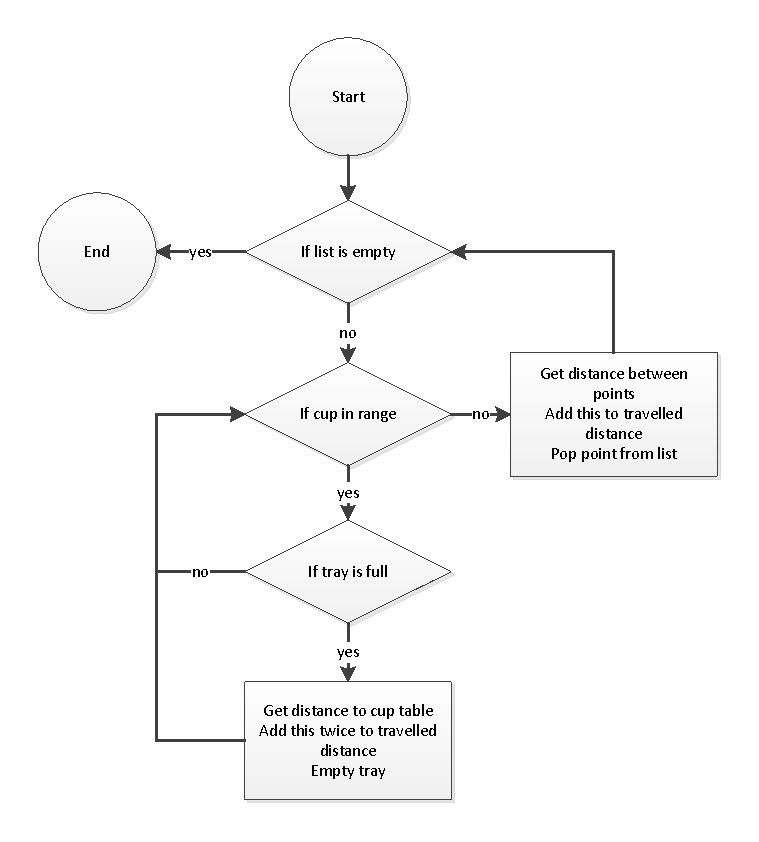
\includegraphics[width=\textwidth,trim=0 0 0 0]{graphics/flowchart.pdf}
	%trim=l b r t (can cut off from every side)
	\caption{Flow chart of the stepper}
	\label{fig:stepper}			
\end{figure}

